\documentclass[twoside]{book}

% Packages required by doxygen
\usepackage{fixltx2e}
\usepackage{calc}
\usepackage{doxygen}
\usepackage[export]{adjustbox} % also loads graphicx
\usepackage{graphicx}
\usepackage[utf8]{inputenc}
\usepackage{makeidx}
\usepackage{multicol}
\usepackage{multirow}
\PassOptionsToPackage{warn}{textcomp}
\usepackage{textcomp}
\usepackage[nointegrals]{wasysym}
\usepackage[table]{xcolor}

% Font selection
\usepackage[T1]{fontenc}
\usepackage[scaled=.90]{helvet}
\usepackage{courier}
\usepackage{amssymb}
\usepackage{sectsty}
\renewcommand{\familydefault}{\sfdefault}
\allsectionsfont{%
  \fontseries{bc}\selectfont%
  \color{darkgray}%
}
\renewcommand{\DoxyLabelFont}{%
  \fontseries{bc}\selectfont%
  \color{darkgray}%
}
\newcommand{\+}{\discretionary{\mbox{\scriptsize$\hookleftarrow$}}{}{}}

% Page & text layout
\usepackage{geometry}
\geometry{%
  a4paper,%
  top=2.5cm,%
  bottom=2.5cm,%
  left=2.5cm,%
  right=2.5cm%
}
\tolerance=750
\hfuzz=15pt
\hbadness=750
\setlength{\emergencystretch}{15pt}
\setlength{\parindent}{0cm}
\setlength{\parskip}{0.2cm}
\makeatletter
\renewcommand{\paragraph}{%
  \@startsection{paragraph}{4}{0ex}{-1.0ex}{1.0ex}{%
    \normalfont\normalsize\bfseries\SS@parafont%
  }%
}
\renewcommand{\subparagraph}{%
  \@startsection{subparagraph}{5}{0ex}{-1.0ex}{1.0ex}{%
    \normalfont\normalsize\bfseries\SS@subparafont%
  }%
}
\makeatother

% Headers & footers
\usepackage{fancyhdr}
\pagestyle{fancyplain}
\fancyhead[LE]{\fancyplain{}{\bfseries\thepage}}
\fancyhead[CE]{\fancyplain{}{}}
\fancyhead[RE]{\fancyplain{}{\bfseries\leftmark}}
\fancyhead[LO]{\fancyplain{}{\bfseries\rightmark}}
\fancyhead[CO]{\fancyplain{}{}}
\fancyhead[RO]{\fancyplain{}{\bfseries\thepage}}
\fancyfoot[LE]{\fancyplain{}{}}
\fancyfoot[CE]{\fancyplain{}{}}
\fancyfoot[RE]{\fancyplain{}{\bfseries\scriptsize Generated on Tue Nov 3 2015 12\+:38\+:12 for Age of Espionage by Doxygen }}
\fancyfoot[LO]{\fancyplain{}{\bfseries\scriptsize Generated on Tue Nov 3 2015 12\+:38\+:12 for Age of Espionage by Doxygen }}
\fancyfoot[CO]{\fancyplain{}{}}
\fancyfoot[RO]{\fancyplain{}{}}
\renewcommand{\footrulewidth}{0.4pt}
\renewcommand{\chaptermark}[1]{%
  \markboth{#1}{}%
}
\renewcommand{\sectionmark}[1]{%
  \markright{\thesection\ #1}%
}

% Indices & bibliography
\usepackage{natbib}
\usepackage[titles]{tocloft}
\setcounter{tocdepth}{3}
\setcounter{secnumdepth}{5}
\makeindex

% Hyperlinks (required, but should be loaded last)
\usepackage{ifpdf}
\ifpdf
  \usepackage[pdftex,pagebackref=true]{hyperref}
\else
  \usepackage[ps2pdf,pagebackref=true]{hyperref}
\fi
\hypersetup{%
  colorlinks=true,%
  linkcolor=blue,%
  citecolor=blue,%
  unicode%
}

% Custom commands
\newcommand{\clearemptydoublepage}{%
  \newpage{\pagestyle{empty}\cleardoublepage}%
}


%===== C O N T E N T S =====

\begin{document}

% Titlepage & ToC
\hypersetup{pageanchor=false,
             bookmarks=true,
             bookmarksnumbered=true,
             pdfencoding=unicode
            }
\pagenumbering{roman}
\begin{titlepage}
\vspace*{7cm}
\begin{center}%
{\Large Age of Espionage \\[1ex]\large 0.\+0.\+1.\+2 }\\
\vspace*{1cm}
{\large Generated by Doxygen 1.8.10}\\
\vspace*{0.5cm}
{\small Tue Nov 3 2015 12:38:12}\\
\end{center}
\end{titlepage}
\clearemptydoublepage
\tableofcontents
\clearemptydoublepage
\pagenumbering{arabic}
\hypersetup{pageanchor=true}

%--- Begin generated contents ---
\chapter{Hierarchical Index}
\section{Class Hierarchy}
This inheritance list is sorted roughly, but not completely, alphabetically\+:\begin{DoxyCompactList}
\item Drawable\begin{DoxyCompactList}
\item \contentsline{section}{helios\+:\+:Base\+Obj}{\pageref{classhelios_1_1_base_obj}}{}
\begin{DoxyCompactList}
\item \contentsline{section}{helios\+:\+:Spr\+Obj}{\pageref{classhelios_1_1_spr_obj}}{}
\begin{DoxyCompactList}
\item \contentsline{section}{aoe\+:\+:Unit}{\pageref{classaoe_1_1_unit}}{}
\end{DoxyCompactList}
\end{DoxyCompactList}
\item \contentsline{section}{helios\+:\+:Room}{\pageref{classhelios_1_1_room}}{}
\end{DoxyCompactList}
\item \contentsline{section}{helios\+:\+:Quad\+Tree}{\pageref{classhelios_1_1_quad_tree}}{}
\end{DoxyCompactList}

\chapter{Class Index}
\section{Class List}
Here are the classes, structs, unions and interfaces with brief descriptions\+:\begin{DoxyCompactList}
\item\contentsline{section}{\hyperlink{classhelios_1_1_base_obj}{helios\+::\+Base\+Obj} \\*An abstract class representing an interface all objects should adhere to }{\pageref{classhelios_1_1_base_obj}}{}
\item\contentsline{section}{\hyperlink{classhelios_1_1_quad_tree}{helios\+::\+Quad\+Tree} }{\pageref{classhelios_1_1_quad_tree}}{}
\item\contentsline{section}{\hyperlink{classhelios_1_1_room}{helios\+::\+Room} \\*Describes a given space and the objects that exist within it in a way that facilitates consistent generation. Rooms are also responsible for calling update routines regularly, checking for collisions, and drawing objects }{\pageref{classhelios_1_1_room}}{}
\item\contentsline{section}{\hyperlink{classhelios_1_1_spr_obj}{helios\+::\+Spr\+Obj} \\*An abstract parent class providing the basis for packaging sprite with the appropriate logic functions all objects in the room need }{\pageref{classhelios_1_1_spr_obj}}{}
\item\contentsline{section}{\hyperlink{classaoe_1_1_unit}{aoe\+::\+Unit} }{\pageref{classaoe_1_1_unit}}{}
\end{DoxyCompactList}

\chapter{Class Documentation}
\hypertarget{class_helios_1_1_base_obj}{}\section{Helios\+:\+:Base\+Obj Class Reference}
\label{class_helios_1_1_base_obj}\index{Helios\+::\+Base\+Obj@{Helios\+::\+Base\+Obj}}


An abstract class representing an interface all objects should adhere to.  




{\ttfamily \#include $<$helios\+\_\+baseobj.\+h$>$}

Inheritance diagram for Helios\+:\+:Base\+Obj\+:\begin{figure}[H]
\begin{center}
\leavevmode
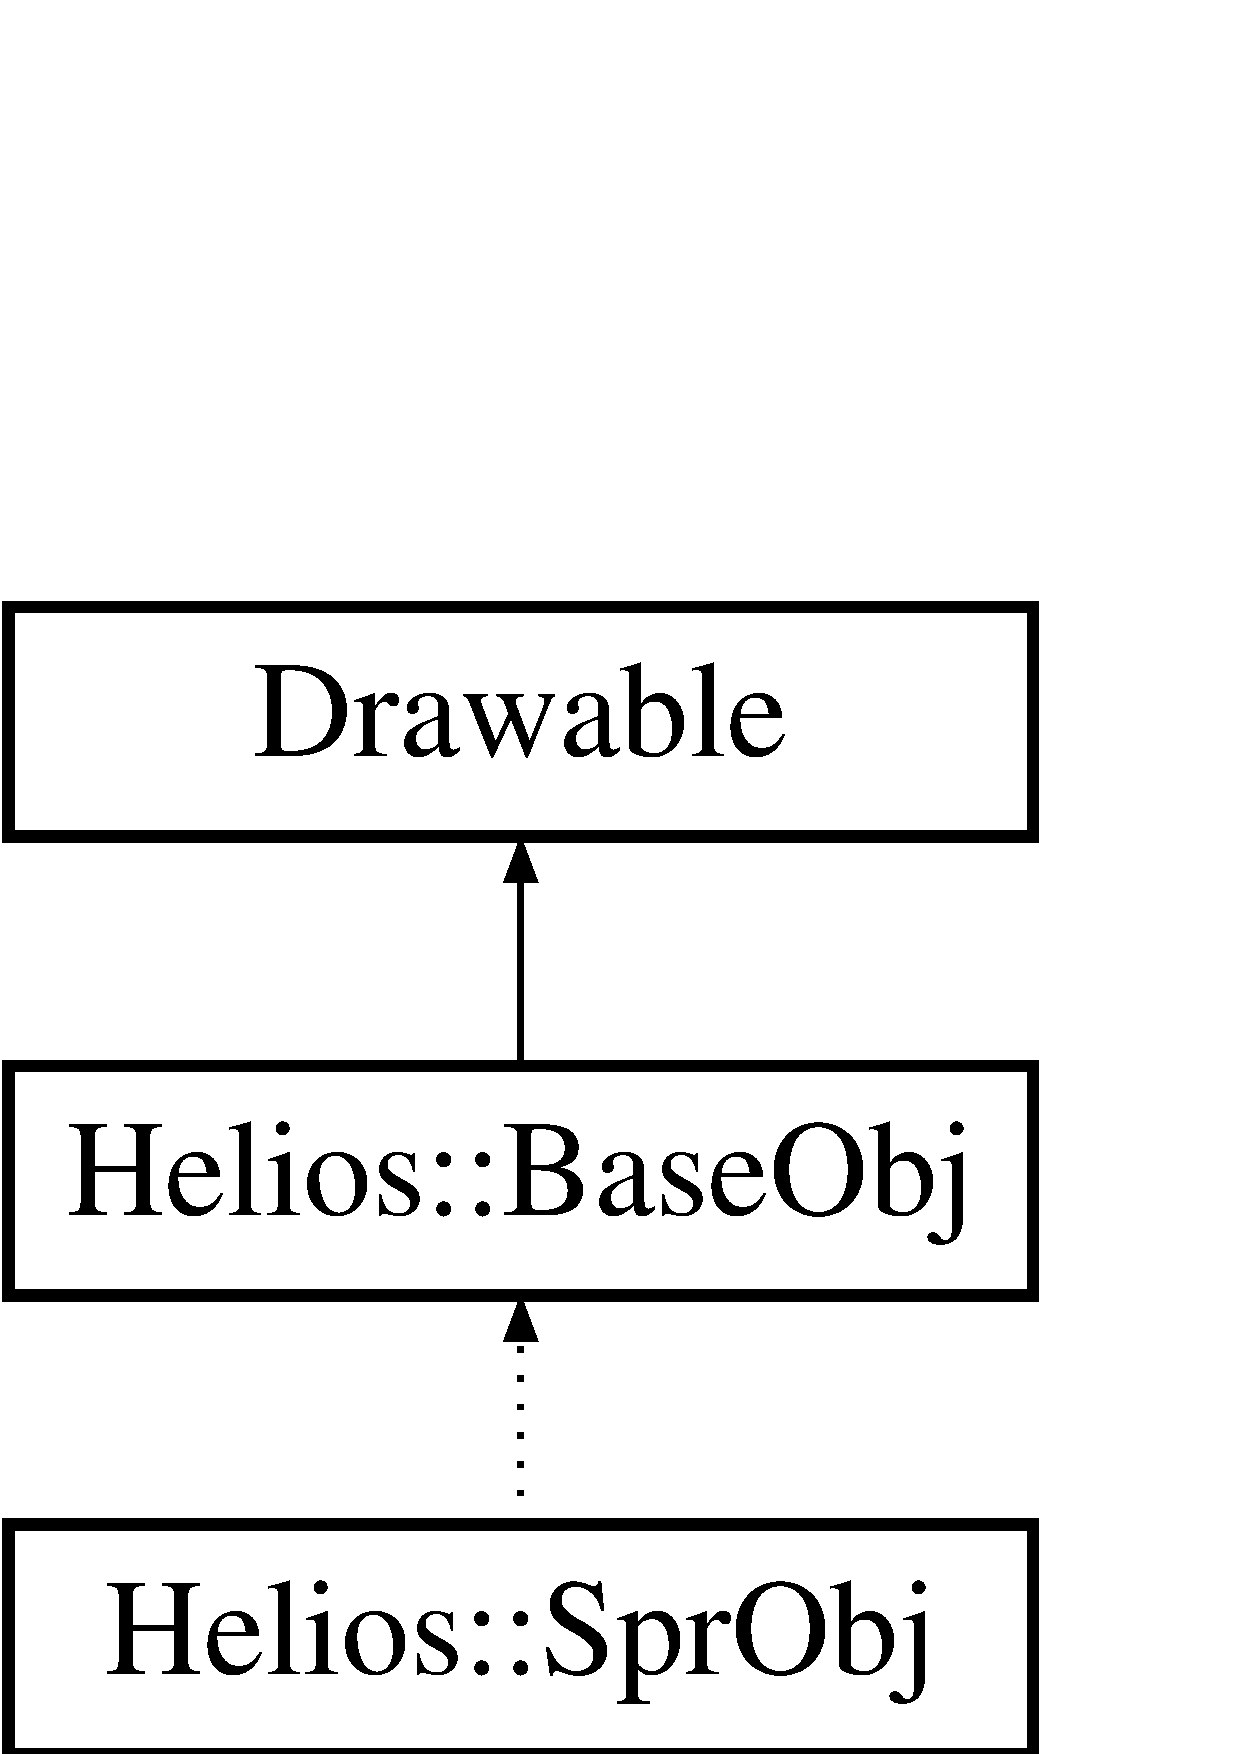
\includegraphics[height=3.000000cm]{class_helios_1_1_base_obj}
\end{center}
\end{figure}
\subsection*{Public Member Functions}
\begin{DoxyCompactItemize}
\item 
\hypertarget{class_helios_1_1_base_obj_aa278e49125c0c84d26906ae47cfff727}{}{\bfseries Base\+Obj} (const \hyperlink{class_helios_1_1_base_obj}{Base\+Obj} \&other)=delete\label{class_helios_1_1_base_obj_aa278e49125c0c84d26906ae47cfff727}

\item 
\hypertarget{class_helios_1_1_base_obj_ad2127aa4f505b6183a9d91d384062b98}{}{\bfseries Base\+Obj} (\hyperlink{class_helios_1_1_base_obj}{Base\+Obj} \&\&other)=delete\label{class_helios_1_1_base_obj_ad2127aa4f505b6183a9d91d384062b98}

\item 
\hypertarget{class_helios_1_1_base_obj_a286cd12e5193430bb3ef554aac0152d9}{}virtual \hyperlink{class_helios_1_1_base_obj_a286cd12e5193430bb3ef554aac0152d9}{$\sim$\+Base\+Obj} ()\label{class_helios_1_1_base_obj_a286cd12e5193430bb3ef554aac0152d9}

\begin{DoxyCompactList}\small\item\em Virtual Destructor. \end{DoxyCompactList}\item 
\hypertarget{class_helios_1_1_base_obj_a499a49d6f7f7f79190e6d598eab4391e}{}\hyperlink{class_helios_1_1_base_obj}{Base\+Obj} \& {\bfseries operator=} (const \hyperlink{class_helios_1_1_base_obj}{Base\+Obj} \&other)=delete\label{class_helios_1_1_base_obj_a499a49d6f7f7f79190e6d598eab4391e}

\item 
\hypertarget{class_helios_1_1_base_obj_ab588e3ffe972a53de418f50558651f2f}{}\hyperlink{class_helios_1_1_base_obj}{Base\+Obj} \& {\bfseries operator=} (\hyperlink{class_helios_1_1_base_obj}{Base\+Obj} \&\&other)=delete\label{class_helios_1_1_base_obj_ab588e3ffe972a53de418f50558651f2f}

\item 
\hyperlink{class_helios_1_1_room}{Room} $\ast$ \hyperlink{class_helios_1_1_base_obj_a896030076cb96c794f4b202cca0ec584}{get\+\_\+room} () const 
\begin{DoxyCompactList}\small\item\em Returns a pointer to the room this object is active in. \end{DoxyCompactList}\item 
signed int \hyperlink{class_helios_1_1_base_obj_abf2a6d187e1c8329bb8e24256218aecb}{get\+\_\+priority} () const 
\begin{DoxyCompactList}\small\item\em Returns the current priority of this object. \end{DoxyCompactList}\item 
bool \hyperlink{class_helios_1_1_base_obj_a418fb8f5e8aa25f0969e37e24cadb8c9}{is\+\_\+visible} () const 
\begin{DoxyCompactList}\small\item\em Checks if the object is visible. \end{DoxyCompactList}\item 
bool \hyperlink{class_helios_1_1_base_obj_a8c748b30dca39c303e8bb9085f9d6d15}{is\+\_\+active} () const 
\begin{DoxyCompactList}\small\item\em Returns whether the Base\+Object is active in any \hyperlink{class_helios_1_1_room}{Room}. \end{DoxyCompactList}\item 
void \hyperlink{class_helios_1_1_base_obj_a0d168130905c7e573ef0a69b53b73bed}{Activate} (\hyperlink{class_helios_1_1_room}{Room} $\ast$room\+Ptr)
\begin{DoxyCompactList}\small\item\em Activates the object, making a \hyperlink{class_helios_1_1_room}{Room} responsible for managing it. \end{DoxyCompactList}\item 
void \hyperlink{class_helios_1_1_base_obj_ade0a810a861f41a43adf0e7c766951d1}{Deactivate} ()
\begin{DoxyCompactList}\small\item\em Deactivates the object, removing all responsibilities of the \hyperlink{class_helios_1_1_room}{Room} it is in. \end{DoxyCompactList}\item 
void \hyperlink{class_helios_1_1_base_obj_a354767a20905778fefe96fe895a382ae}{set\+\_\+visible} (const bool vis)
\begin{DoxyCompactList}\small\item\em Sets the visibility of the object. \end{DoxyCompactList}\item 
virtual void \hyperlink{class_helios_1_1_base_obj_aa42e26e872234b6871d159c29afdef17}{Update} ()=0
\begin{DoxyCompactList}\small\item\em Virtual Update Function. \end{DoxyCompactList}\end{DoxyCompactItemize}
\subsection*{Protected Member Functions}
\begin{DoxyCompactItemize}
\item 
\hyperlink{class_helios_1_1_base_obj_ad77bdec51d537c1bfc9661b728980498}{Base\+Obj} (const unsigned int priority=0)
\begin{DoxyCompactList}\small\item\em Default Constructor. \end{DoxyCompactList}\item 
virtual void \hyperlink{class_helios_1_1_base_obj_af7355477f06d38692dc6cdb6f99dbd11}{render} (sf\+::\+Render\+Target \&target, sf\+::\+Render\+States states) const  =0
\begin{DoxyCompactList}\small\item\em Draw the object to a render target. \end{DoxyCompactList}\end{DoxyCompactItemize}
\subsection*{Protected Attributes}
\begin{DoxyCompactItemize}
\item 
signed int \hyperlink{class_helios_1_1_base_obj_aad807d0a4296ffdfddf2e653b428481a}{\+\_\+priority}
\begin{DoxyCompactList}\small\item\em The priority of this object\textquotesingle{}s update() and draw() calls. \end{DoxyCompactList}\item 
bool \hyperlink{class_helios_1_1_base_obj_aed78a9a68c038e6d82e07711f9065e33}{\+\_\+visible}
\begin{DoxyCompactList}\small\item\em Flag denoting visibility. \end{DoxyCompactList}\end{DoxyCompactItemize}


\subsection{Detailed Description}
An abstract class representing an interface all objects should adhere to. 

\hyperlink{class_helios_1_1_base_obj}{Base\+Obj} is merely defines interface for all objects. Thus, all objects should have an Update function, which is inteded to be called on the object for each game step.~\newline
~\newline
 All objects are also sf\+::\+Drawables, and will only draw if they are visible. Specify how to draw derived classes with the virtual function render in order to maintain visible functionality.~\newline
~\newline
 Objects are also designed to be managed by the \hyperlink{class_helios_1_1_room}{Room} class. For this reason, they may be set as active in a room using the Activate function. This will inform both parties that the \hyperlink{class_helios_1_1_room}{Room} in question is responsible for managing Update and draw function calls as well as interactions between objects in the \hyperlink{class_helios_1_1_room}{Room}.~\newline


\subsection{Constructor \& Destructor Documentation}
\hypertarget{class_helios_1_1_base_obj_ad77bdec51d537c1bfc9661b728980498}{}\index{Helios\+::\+Base\+Obj@{Helios\+::\+Base\+Obj}!Base\+Obj@{Base\+Obj}}
\index{Base\+Obj@{Base\+Obj}!Helios\+::\+Base\+Obj@{Helios\+::\+Base\+Obj}}
\subsubsection[{Base\+Obj(const unsigned int priority=0)}]{\setlength{\rightskip}{0pt plus 5cm}Base\+Obj\+::\+Base\+Obj (
\begin{DoxyParamCaption}
\item[{const unsigned int}]{priority = {\ttfamily 0}}
\end{DoxyParamCaption}
)\hspace{0.3cm}{\ttfamily [explicit]}, {\ttfamily [protected]}}\label{class_helios_1_1_base_obj_ad77bdec51d537c1bfc9661b728980498}


Default Constructor. 

Creates an object that is inactive and invisible, with the given priority (default zero).


\begin{DoxyParams}{Parameters}
{\em priority} & Priority of object \\
\hline
\end{DoxyParams}


\subsection{Member Function Documentation}
\hypertarget{class_helios_1_1_base_obj_a0d168130905c7e573ef0a69b53b73bed}{}\index{Helios\+::\+Base\+Obj@{Helios\+::\+Base\+Obj}!Activate@{Activate}}
\index{Activate@{Activate}!Helios\+::\+Base\+Obj@{Helios\+::\+Base\+Obj}}
\subsubsection[{Activate(\+Room $\ast$room\+Ptr)}]{\setlength{\rightskip}{0pt plus 5cm}void Base\+Obj\+::\+Activate (
\begin{DoxyParamCaption}
\item[{{\bf Room} $\ast$}]{room\+Ptr}
\end{DoxyParamCaption}
)}\label{class_helios_1_1_base_obj_a0d168130905c7e573ef0a69b53b73bed}


Activates the object, making a \hyperlink{class_helios_1_1_room}{Room} responsible for managing it. 

The \hyperlink{class_helios_1_1_room}{Room} responsible for this object will call update each step, draw each frame, and may optimize other object interactions such as collision checks.


\begin{DoxyParams}{Parameters}
{\em room\+Ptr} & A pointer to the \hyperlink{class_helios_1_1_room}{Room} to activate in\\
\hline
\end{DoxyParams}
\begin{DoxyPrecond}{Precondition}
The object is not active 
\end{DoxyPrecond}
\begin{DoxyPostcond}{Postcondition}
The object is active
\end{DoxyPostcond}
\begin{DoxySeeAlso}{See also}
\hyperlink{class_helios_1_1_base_obj_a8c748b30dca39c303e8bb9085f9d6d15}{is\+\_\+active()}, \hyperlink{class_helios_1_1_base_obj_ade0a810a861f41a43adf0e7c766951d1}{Deactivate()} 
\end{DoxySeeAlso}
\hypertarget{class_helios_1_1_base_obj_ade0a810a861f41a43adf0e7c766951d1}{}\index{Helios\+::\+Base\+Obj@{Helios\+::\+Base\+Obj}!Deactivate@{Deactivate}}
\index{Deactivate@{Deactivate}!Helios\+::\+Base\+Obj@{Helios\+::\+Base\+Obj}}
\subsubsection[{Deactivate()}]{\setlength{\rightskip}{0pt plus 5cm}void Base\+Obj\+::\+Deactivate (
\begin{DoxyParamCaption}
{}
\end{DoxyParamCaption}
)}\label{class_helios_1_1_base_obj_ade0a810a861f41a43adf0e7c766951d1}


Deactivates the object, removing all responsibilities of the \hyperlink{class_helios_1_1_room}{Room} it is in. 

Deactivating an object

\begin{DoxyPrecond}{Precondition}
The object is active 
\end{DoxyPrecond}
\begin{DoxyPostcond}{Postcondition}
The object is not active
\end{DoxyPostcond}
\begin{DoxySeeAlso}{See also}
\hyperlink{class_helios_1_1_base_obj_a8c748b30dca39c303e8bb9085f9d6d15}{is\+\_\+active()}, Activate(\+Room \&room\+Handle) 
\end{DoxySeeAlso}
\hypertarget{class_helios_1_1_base_obj_abf2a6d187e1c8329bb8e24256218aecb}{}\index{Helios\+::\+Base\+Obj@{Helios\+::\+Base\+Obj}!get\+\_\+priority@{get\+\_\+priority}}
\index{get\+\_\+priority@{get\+\_\+priority}!Helios\+::\+Base\+Obj@{Helios\+::\+Base\+Obj}}
\subsubsection[{get\+\_\+priority() const }]{\setlength{\rightskip}{0pt plus 5cm}signed int Base\+Obj\+::get\+\_\+priority (
\begin{DoxyParamCaption}
{}
\end{DoxyParamCaption}
) const}\label{class_helios_1_1_base_obj_abf2a6d187e1c8329bb8e24256218aecb}


Returns the current priority of this object. 

The object\textquotesingle{}s priority represents how early in the update cycle this object\textquotesingle{}s \hyperlink{class_helios_1_1_base_obj_aa42e26e872234b6871d159c29afdef17}{Update()} and draw() calls should be made. Given two objects, the object with the higher priority should be updated and drawn before the other.

\begin{DoxyReturn}{Returns}
signed int priority.
\end{DoxyReturn}
\begin{DoxySeeAlso}{See also}
set\+\_\+priority() 
\end{DoxySeeAlso}
\hypertarget{class_helios_1_1_base_obj_a896030076cb96c794f4b202cca0ec584}{}\index{Helios\+::\+Base\+Obj@{Helios\+::\+Base\+Obj}!get\+\_\+room@{get\+\_\+room}}
\index{get\+\_\+room@{get\+\_\+room}!Helios\+::\+Base\+Obj@{Helios\+::\+Base\+Obj}}
\subsubsection[{get\+\_\+room() const }]{\setlength{\rightskip}{0pt plus 5cm}{\bf Room} $\ast$ Base\+Obj\+::get\+\_\+room (
\begin{DoxyParamCaption}
{}
\end{DoxyParamCaption}
) const}\label{class_helios_1_1_base_obj_a896030076cb96c794f4b202cca0ec584}


Returns a pointer to the room this object is active in. 

Inactive objects return nullptr.

\begin{DoxyReturn}{Returns}
Room$\ast$ handle 
\end{DoxyReturn}
\hypertarget{class_helios_1_1_base_obj_a8c748b30dca39c303e8bb9085f9d6d15}{}\index{Helios\+::\+Base\+Obj@{Helios\+::\+Base\+Obj}!is\+\_\+active@{is\+\_\+active}}
\index{is\+\_\+active@{is\+\_\+active}!Helios\+::\+Base\+Obj@{Helios\+::\+Base\+Obj}}
\subsubsection[{is\+\_\+active() const }]{\setlength{\rightskip}{0pt plus 5cm}bool Base\+Obj\+::is\+\_\+active (
\begin{DoxyParamCaption}
{}
\end{DoxyParamCaption}
) const}\label{class_helios_1_1_base_obj_a8c748b30dca39c303e8bb9085f9d6d15}


Returns whether the Base\+Object is active in any \hyperlink{class_helios_1_1_room}{Room}. 

Active objects are linked to some \hyperlink{class_helios_1_1_room}{Room} which is held responsible for calling Update and draw regularly as well as enabling other functionality such as collision checks with other objects in the \hyperlink{class_helios_1_1_room}{Room}. ~\newline
~\newline
 An object can only be active in one \hyperlink{class_helios_1_1_room}{Room} at a time.

\begin{DoxyReturn}{Returns}
bool active
\end{DoxyReturn}
\begin{DoxySeeAlso}{See also}
Activate(\+Room \&room\+Handle), \hyperlink{class_helios_1_1_base_obj_ade0a810a861f41a43adf0e7c766951d1}{Deactivate()} 
\end{DoxySeeAlso}
\hypertarget{class_helios_1_1_base_obj_a418fb8f5e8aa25f0969e37e24cadb8c9}{}\index{Helios\+::\+Base\+Obj@{Helios\+::\+Base\+Obj}!is\+\_\+visible@{is\+\_\+visible}}
\index{is\+\_\+visible@{is\+\_\+visible}!Helios\+::\+Base\+Obj@{Helios\+::\+Base\+Obj}}
\subsubsection[{is\+\_\+visible() const }]{\setlength{\rightskip}{0pt plus 5cm}bool Base\+Obj\+::is\+\_\+visible (
\begin{DoxyParamCaption}
{}
\end{DoxyParamCaption}
) const}\label{class_helios_1_1_base_obj_a418fb8f5e8aa25f0969e37e24cadb8c9}


Checks if the object is visible. 

If an object is not visible, then calls to draw that object will be ignored.

\begin{DoxyReturn}{Returns}
bool visible
\end{DoxyReturn}
\begin{DoxySeeAlso}{See also}
\hyperlink{class_helios_1_1_base_obj_a354767a20905778fefe96fe895a382ae}{set\+\_\+visible()} 
\end{DoxySeeAlso}
\hypertarget{class_helios_1_1_base_obj_af7355477f06d38692dc6cdb6f99dbd11}{}\index{Helios\+::\+Base\+Obj@{Helios\+::\+Base\+Obj}!render@{render}}
\index{render@{render}!Helios\+::\+Base\+Obj@{Helios\+::\+Base\+Obj}}
\subsubsection[{render(sf\+::\+Render\+Target \&target, sf\+::\+Render\+States states) const  =0}]{\setlength{\rightskip}{0pt plus 5cm}virtual void Helios\+::\+Base\+Obj\+::render (
\begin{DoxyParamCaption}
\item[{sf\+::\+Render\+Target \&}]{target, }
\item[{sf\+::\+Render\+States}]{states}
\end{DoxyParamCaption}
) const\hspace{0.3cm}{\ttfamily [protected]}, {\ttfamily [pure virtual]}}\label{class_helios_1_1_base_obj_af7355477f06d38692dc6cdb6f99dbd11}


Draw the object to a render target. 

This is a pure virtual function that has to be implemented by the derived class to define how the object should be drawn.


\begin{DoxyParams}{Parameters}
{\em target} & Render target to draw to. \\
\hline
{\em states} & Current render states. \\
\hline
\end{DoxyParams}


Implemented in \hyperlink{class_helios_1_1_spr_obj_a9f21ff22d40d1f06dc58fbc9b2b16de7}{Helios\+::\+Spr\+Obj}.

\hypertarget{class_helios_1_1_base_obj_a354767a20905778fefe96fe895a382ae}{}\index{Helios\+::\+Base\+Obj@{Helios\+::\+Base\+Obj}!set\+\_\+visible@{set\+\_\+visible}}
\index{set\+\_\+visible@{set\+\_\+visible}!Helios\+::\+Base\+Obj@{Helios\+::\+Base\+Obj}}
\subsubsection[{set\+\_\+visible(const bool vis)}]{\setlength{\rightskip}{0pt plus 5cm}void Base\+Obj\+::set\+\_\+visible (
\begin{DoxyParamCaption}
\item[{const bool}]{vis}
\end{DoxyParamCaption}
)}\label{class_helios_1_1_base_obj_a354767a20905778fefe96fe895a382ae}


Sets the visibility of the object. 


\begin{DoxyParams}{Parameters}
{\em vis} & Desired visibility\\
\hline
\end{DoxyParams}
\begin{DoxySeeAlso}{See also}
\hyperlink{class_helios_1_1_base_obj_a418fb8f5e8aa25f0969e37e24cadb8c9}{is\+\_\+visible()} 
\end{DoxySeeAlso}
\hypertarget{class_helios_1_1_base_obj_aa42e26e872234b6871d159c29afdef17}{}\index{Helios\+::\+Base\+Obj@{Helios\+::\+Base\+Obj}!Update@{Update}}
\index{Update@{Update}!Helios\+::\+Base\+Obj@{Helios\+::\+Base\+Obj}}
\subsubsection[{Update()=0}]{\setlength{\rightskip}{0pt plus 5cm}virtual void Helios\+::\+Base\+Obj\+::\+Update (
\begin{DoxyParamCaption}
{}
\end{DoxyParamCaption}
)\hspace{0.3cm}{\ttfamily [pure virtual]}}\label{class_helios_1_1_base_obj_aa42e26e872234b6871d159c29afdef17}


Virtual Update Function. 

This function should hold the code defining how to update after each game step. It will likelly be different for each derived class. 

Implemented in \hyperlink{class_helios_1_1_spr_obj_a5ea59f62cf7bb7bd7ff8080a79894037}{Helios\+::\+Spr\+Obj}.



\subsection{Member Data Documentation}
\hypertarget{class_helios_1_1_base_obj_aad807d0a4296ffdfddf2e653b428481a}{}\index{Helios\+::\+Base\+Obj@{Helios\+::\+Base\+Obj}!\+\_\+priority@{\+\_\+priority}}
\index{\+\_\+priority@{\+\_\+priority}!Helios\+::\+Base\+Obj@{Helios\+::\+Base\+Obj}}
\subsubsection[{\+\_\+priority}]{\setlength{\rightskip}{0pt plus 5cm}signed int Helios\+::\+Base\+Obj\+::\+\_\+priority\hspace{0.3cm}{\ttfamily [protected]}}\label{class_helios_1_1_base_obj_aad807d0a4296ffdfddf2e653b428481a}


The priority of this object\textquotesingle{}s update() and draw() calls. 

Priority is relative. Between two objects in the same \hyperlink{class_helios_1_1_room}{Room}, the object with the higher \+\_\+priority will be updated and drawn first. It is expected that the object itself will know what the ideal priority is for it at any moment. \hypertarget{class_helios_1_1_base_obj_aed78a9a68c038e6d82e07711f9065e33}{}\index{Helios\+::\+Base\+Obj@{Helios\+::\+Base\+Obj}!\+\_\+visible@{\+\_\+visible}}
\index{\+\_\+visible@{\+\_\+visible}!Helios\+::\+Base\+Obj@{Helios\+::\+Base\+Obj}}
\subsubsection[{\+\_\+visible}]{\setlength{\rightskip}{0pt plus 5cm}bool Helios\+::\+Base\+Obj\+::\+\_\+visible\hspace{0.3cm}{\ttfamily [protected]}}\label{class_helios_1_1_base_obj_aed78a9a68c038e6d82e07711f9065e33}


Flag denoting visibility. 

If \+\_\+visible is false, drawing will be prevented. 

The documentation for this class was generated from the following files\+:\begin{DoxyCompactItemize}
\item 
S\+F\+M\+L\+Game/\+Helios/helios\+\_\+baseobj.\+h\item 
S\+F\+M\+L\+Game/\+Helios/helios\+\_\+baseobj.\+cpp\end{DoxyCompactItemize}

\hypertarget{class_helios_1_1_quad_tree}{}\section{Helios\+:\+:Quad\+Tree Class Reference}
\label{class_helios_1_1_quad_tree}\index{Helios\+::\+Quad\+Tree@{Helios\+::\+Quad\+Tree}}
\subsection*{Public Member Functions}
\begin{DoxyCompactItemize}
\item 
\hypertarget{class_helios_1_1_quad_tree_afe790179e3b622d2b2bbb2d431c167bc}{}{\bfseries Quad\+Tree} (const \hyperlink{class_helios_1_1_quad_tree}{Quad\+Tree} \&other)\label{class_helios_1_1_quad_tree_afe790179e3b622d2b2bbb2d431c167bc}

\item 
\hypertarget{class_helios_1_1_quad_tree_a9a40d641d5011e667259fae1ba833d67}{}{\bfseries Quad\+Tree} (\hyperlink{class_helios_1_1_quad_tree}{Quad\+Tree} \&\&other)\label{class_helios_1_1_quad_tree_a9a40d641d5011e667259fae1ba833d67}

\item 
\hypertarget{class_helios_1_1_quad_tree_a01fe5a42db3aa7194e49a2b97fdd5cc2}{}\hyperlink{class_helios_1_1_quad_tree}{Quad\+Tree} {\bfseries operator=} (const \hyperlink{class_helios_1_1_quad_tree}{Quad\+Tree} \&other)\label{class_helios_1_1_quad_tree_a01fe5a42db3aa7194e49a2b97fdd5cc2}

\item 
\hypertarget{class_helios_1_1_quad_tree_a393f1b3d1b351f541593a667d5ba74cb}{}\hyperlink{class_helios_1_1_quad_tree}{Quad\+Tree} {\bfseries operator=} (\hyperlink{class_helios_1_1_quad_tree}{Quad\+Tree} \&\&other)\label{class_helios_1_1_quad_tree_a393f1b3d1b351f541593a667d5ba74cb}

\end{DoxyCompactItemize}


The documentation for this class was generated from the following file\+:\begin{DoxyCompactItemize}
\item 
S\+F\+M\+L\+Game/\+Helios/helios\+\_\+collision.\+h\end{DoxyCompactItemize}

\hypertarget{class_helios_1_1_room}{}\section{Helios\+:\+:Room Class Reference}
\label{class_helios_1_1_room}\index{Helios\+::\+Room@{Helios\+::\+Room}}


{\ttfamily \#include $<$helios\+\_\+room.\+h$>$}

Inheritance diagram for Helios\+:\+:Room\+:\begin{figure}[H]
\begin{center}
\leavevmode
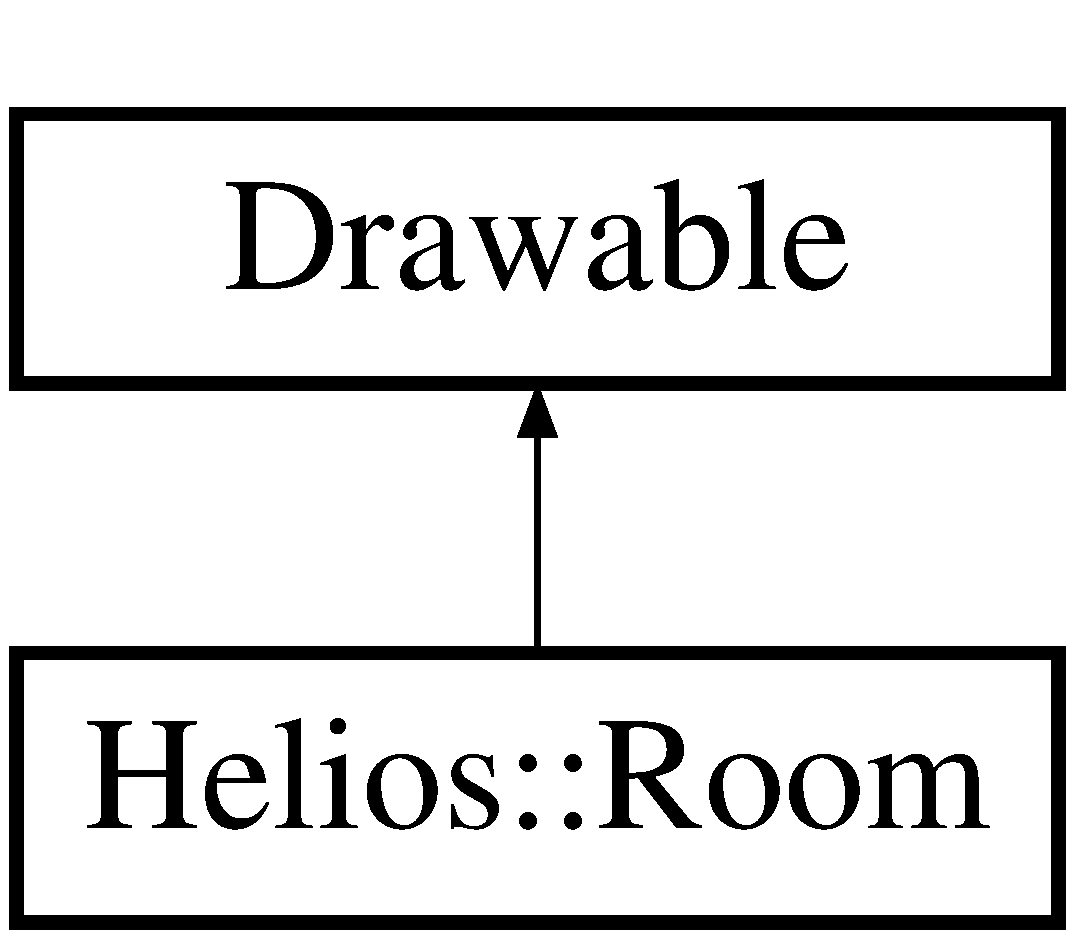
\includegraphics[height=2.000000cm]{class_helios_1_1_room}
\end{center}
\end{figure}
\subsection*{Public Member Functions}
\begin{DoxyCompactItemize}
\item 
\hypertarget{class_helios_1_1_room_adde05da30e6a7923349d3682f77a595e}{}{\bfseries Room} (const \hyperlink{class_helios_1_1_room}{Room} \&other)=delete\label{class_helios_1_1_room_adde05da30e6a7923349d3682f77a595e}

\item 
\hypertarget{class_helios_1_1_room_a49dee88dbca1430546f49dedda0ef88a}{}{\bfseries Room} (\hyperlink{class_helios_1_1_room}{Room} \&\&other)=delete\label{class_helios_1_1_room_a49dee88dbca1430546f49dedda0ef88a}

\item 
\hypertarget{class_helios_1_1_room_a069b54c002742b2e943e281520654d43}{}\hyperlink{class_helios_1_1_room_a069b54c002742b2e943e281520654d43}{Room} (sf\+::\+Vector2u room\+Size)\label{class_helios_1_1_room_a069b54c002742b2e943e281520654d43}

\begin{DoxyCompactList}\small\item\em Constructors \& Destructors\+: \end{DoxyCompactList}\item 
\hypertarget{class_helios_1_1_room_ac4529d35e99e767f434e0c33f922257a}{}\hyperlink{class_helios_1_1_room}{Room} \& {\bfseries operator=} (const \hyperlink{class_helios_1_1_room}{Room} \&other)=delete\label{class_helios_1_1_room_ac4529d35e99e767f434e0c33f922257a}

\item 
\hypertarget{class_helios_1_1_room_a9f5645c1ec1a46c98ee7621c7a327723}{}\hyperlink{class_helios_1_1_room}{Room} \& {\bfseries operator=} (\hyperlink{class_helios_1_1_room}{Room} \&\&other)=delete\label{class_helios_1_1_room_a9f5645c1ec1a46c98ee7621c7a327723}

\item 
\hypertarget{class_helios_1_1_room_a26dd287e7d05d6157b97bd42ca4c5f54}{}sf\+::\+Time {\bfseries Update} ()\label{class_helios_1_1_room_a26dd287e7d05d6157b97bd42ca4c5f54}

\item 
\hypertarget{class_helios_1_1_room_a1dc648407daeb69bed664c1b6aca899d}{}void {\bfseries Link\+Object} (\hyperlink{class_helios_1_1_base_obj}{Base\+Obj} $\ast$obj\+Ptr)\label{class_helios_1_1_room_a1dc648407daeb69bed664c1b6aca899d}

\item 
\hypertarget{class_helios_1_1_room_ae94868797f3224f81604193f7e6e9af0}{}void {\bfseries Unlink\+Object} (\hyperlink{class_helios_1_1_base_obj}{Base\+Obj} $\ast$obj\+Ptr)\label{class_helios_1_1_room_ae94868797f3224f81604193f7e6e9af0}

\end{DoxyCompactItemize}


\subsection{Detailed Description}
Describes a given space and the objects that exist within it in a way that facilitates consistent generation. Rooms are also responsible for calling update routines regularly, checking for collisions, and drawing objects. 

The documentation for this class was generated from the following files\+:\begin{DoxyCompactItemize}
\item 
S\+F\+M\+L\+Game/\+Helios/helios\+\_\+room.\+h\item 
S\+F\+M\+L\+Game/\+Helios/helios\+\_\+room.\+cpp\end{DoxyCompactItemize}

\hypertarget{class_helios_1_1_spr_obj}{}\section{Helios\+:\+:Spr\+Obj Class Reference}
\label{class_helios_1_1_spr_obj}\index{Helios\+::\+Spr\+Obj@{Helios\+::\+Spr\+Obj}}


{\ttfamily \#include $<$helios\+\_\+sprobj.\+h$>$}

Inheritance diagram for Helios\+:\+:Spr\+Obj\+:\begin{figure}[H]
\begin{center}
\leavevmode
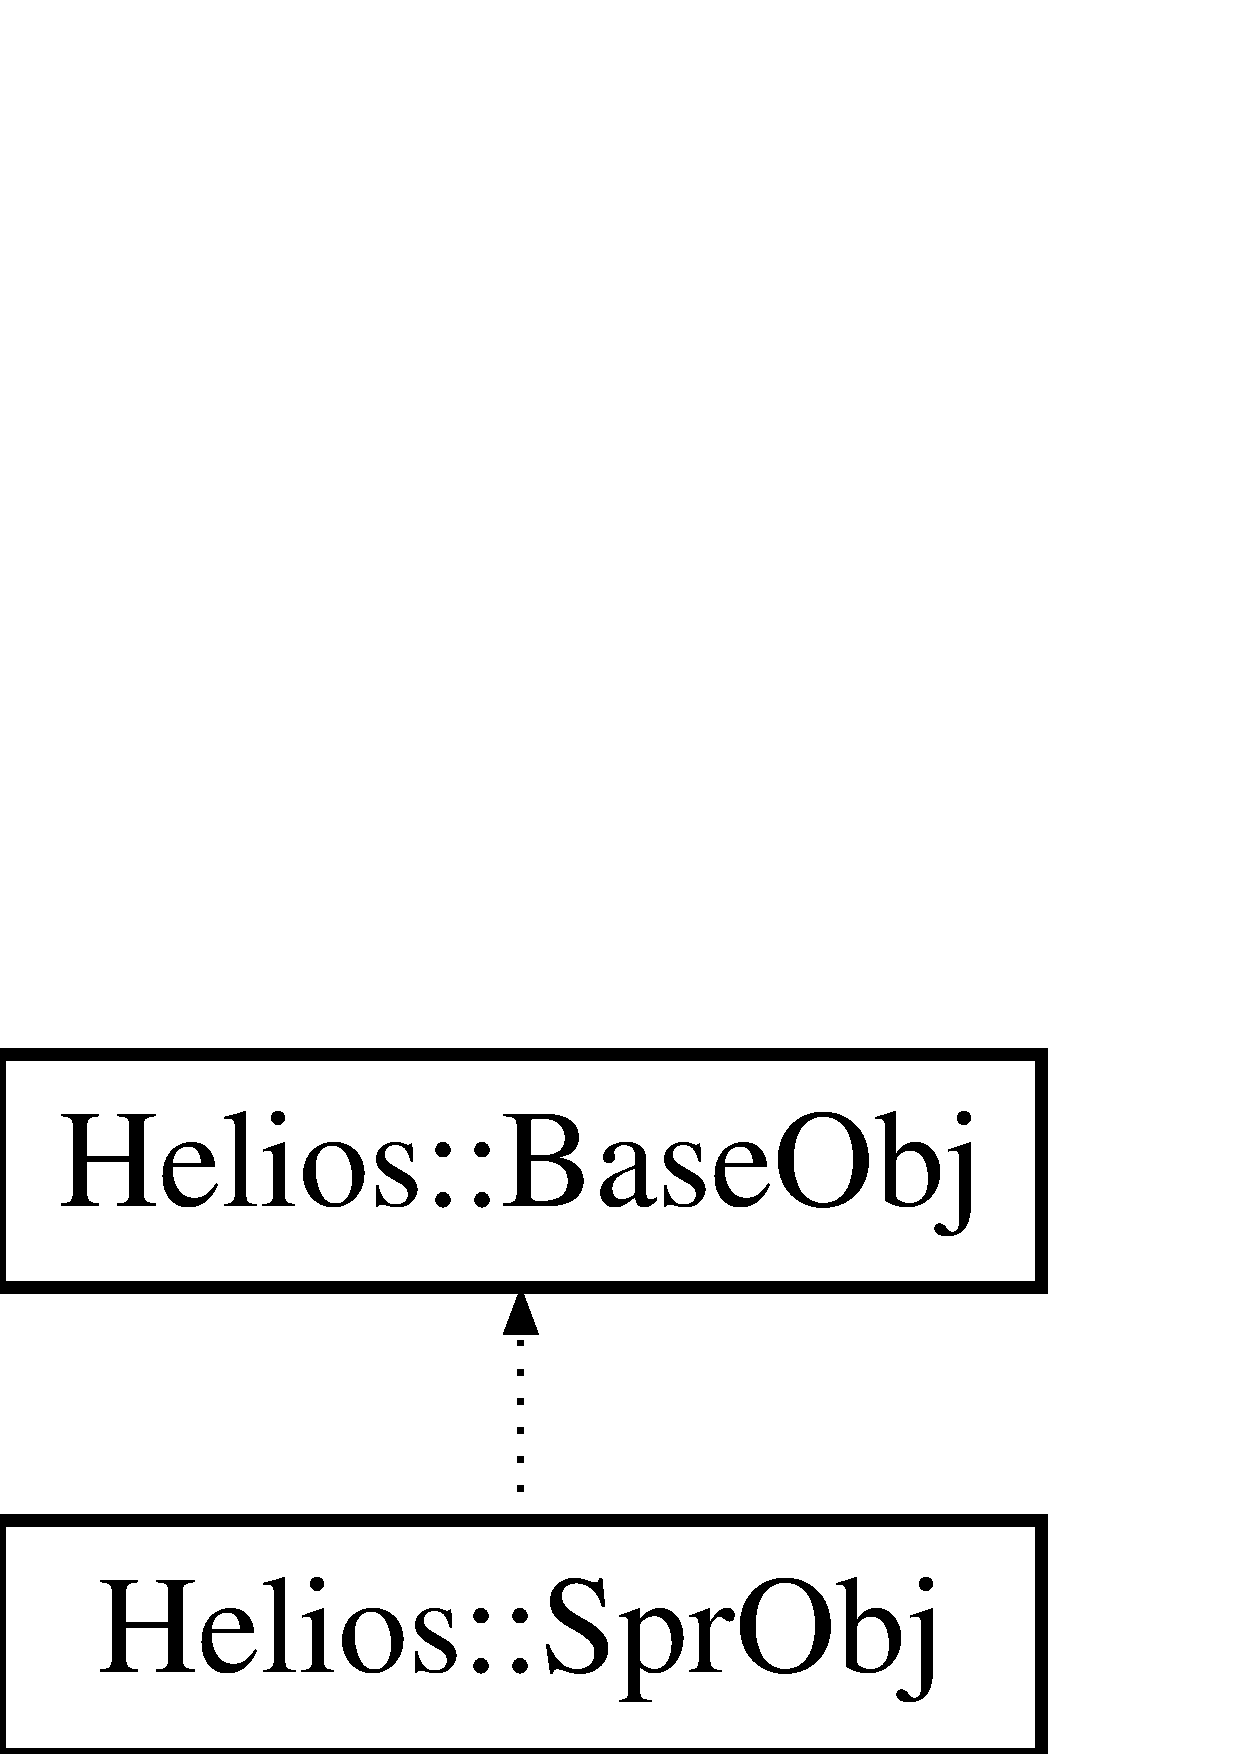
\includegraphics[height=2.000000cm]{class_helios_1_1_spr_obj}
\end{center}
\end{figure}
\subsection*{Public Member Functions}
\begin{DoxyCompactItemize}
\item 
\hypertarget{class_helios_1_1_spr_obj_a25235d4dbfaeda9dfc1c157b2e6ebb05}{}\hyperlink{class_helios_1_1_spr_obj_a25235d4dbfaeda9dfc1c157b2e6ebb05}{Spr\+Obj} (const unsigned int priority=0)\label{class_helios_1_1_spr_obj_a25235d4dbfaeda9dfc1c157b2e6ebb05}

\begin{DoxyCompactList}\small\item\em Constructors and Destructor\+: \end{DoxyCompactList}\item 
\hypertarget{class_helios_1_1_spr_obj_ab803d71e66b25686f4d6a29c1f3ee0d6}{}{\bfseries Spr\+Obj} (const \hyperlink{class_helios_1_1_spr_obj}{Spr\+Obj} \&other)=delete\label{class_helios_1_1_spr_obj_ab803d71e66b25686f4d6a29c1f3ee0d6}

\item 
\hypertarget{class_helios_1_1_spr_obj_ab0a6136a689b13a5ab16270df52a303a}{}{\bfseries Spr\+Obj} (\hyperlink{class_helios_1_1_spr_obj}{Spr\+Obj} \&\&other)=delete\label{class_helios_1_1_spr_obj_ab0a6136a689b13a5ab16270df52a303a}

\item 
\hypertarget{class_helios_1_1_spr_obj_a89e23d41b2a2b4262ed68b9c81cdbe42}{}\hyperlink{class_helios_1_1_base_obj}{Base\+Obj} \& \hyperlink{class_helios_1_1_spr_obj_a89e23d41b2a2b4262ed68b9c81cdbe42}{operator=} (const \hyperlink{class_helios_1_1_base_obj}{Base\+Obj} \&other)=delete\label{class_helios_1_1_spr_obj_a89e23d41b2a2b4262ed68b9c81cdbe42}

\begin{DoxyCompactList}\small\item\em Operators\+: \end{DoxyCompactList}\item 
\hypertarget{class_helios_1_1_spr_obj_a99d676eda512fa5dbc026ca6db1bfcb0}{}\hyperlink{class_helios_1_1_base_obj}{Base\+Obj} \& {\bfseries operator=} (\hyperlink{class_helios_1_1_base_obj}{Base\+Obj} \&\&other)=delete\label{class_helios_1_1_spr_obj_a99d676eda512fa5dbc026ca6db1bfcb0}

\item 
virtual void \hyperlink{class_helios_1_1_spr_obj_a5ea59f62cf7bb7bd7ff8080a79894037}{Update} ()=0
\begin{DoxyCompactList}\small\item\em Step and Frame Functions\+: \end{DoxyCompactList}\end{DoxyCompactItemize}
\subsection*{Protected Member Functions}
\begin{DoxyCompactItemize}
\item 
virtual void \hyperlink{class_helios_1_1_spr_obj_a4cfc26ae9779c15ae4db84e5736cb6b1}{render} (sf\+::\+Render\+Target \&target, sf\+::\+Render\+States states) const  =0
\begin{DoxyCompactList}\small\item\em Proctected Methods. \end{DoxyCompactList}\end{DoxyCompactItemize}
\subsection*{Protected Attributes}
\begin{DoxyCompactItemize}
\item 
\hypertarget{class_helios_1_1_spr_obj_ac9b20866be4703e1285b1b75e2e08490}{}std\+::vector$<$ sf\+::\+Sprite $>$ \hyperlink{class_helios_1_1_spr_obj_ac9b20866be4703e1285b1b75e2e08490}{spr\+Vector}\label{class_helios_1_1_spr_obj_ac9b20866be4703e1285b1b75e2e08490}

\begin{DoxyCompactList}\small\item\em Protected Data. \end{DoxyCompactList}\item 
\hypertarget{class_helios_1_1_spr_obj_a5a5099d52e40625858912ed29c519c59}{}size\+\_\+t {\bfseries spr\+Index}\label{class_helios_1_1_spr_obj_a5a5099d52e40625858912ed29c519c59}

\end{DoxyCompactItemize}


\subsection{Detailed Description}
An abstract parent class providing the basis for packaging sprite with the appropriate logic functions all objects in the room need. 

\subsection{Member Function Documentation}
\hypertarget{class_helios_1_1_spr_obj_a4cfc26ae9779c15ae4db84e5736cb6b1}{}\index{Helios\+::\+Spr\+Obj@{Helios\+::\+Spr\+Obj}!render@{render}}
\index{render@{render}!Helios\+::\+Spr\+Obj@{Helios\+::\+Spr\+Obj}}
\subsubsection[{render(sf\+::\+Render\+Target \&target, sf\+::\+Render\+States states) const  =0}]{\setlength{\rightskip}{0pt plus 5cm}virtual void Helios\+::\+Spr\+Obj\+::render (
\begin{DoxyParamCaption}
\item[{sf\+::\+Render\+Target \&}]{target, }
\item[{sf\+::\+Render\+States}]{states}
\end{DoxyParamCaption}
) const\hspace{0.3cm}{\ttfamily [protected]}, {\ttfamily [pure virtual]}}\label{class_helios_1_1_spr_obj_a4cfc26ae9779c15ae4db84e5736cb6b1}


Proctected Methods. 

Draws the spr\+Index-\/th Sprite in the spr\+Vector.

\begin{DoxyPrecond}{Precondition}
0 $<$= spr\+Vector $<$ spr\+Vector.\+size() 
\end{DoxyPrecond}


Implements \hyperlink{class_helios_1_1_base_obj_af7355477f06d38692dc6cdb6f99dbd11}{Helios\+::\+Base\+Obj}.

\hypertarget{class_helios_1_1_spr_obj_a5ea59f62cf7bb7bd7ff8080a79894037}{}\index{Helios\+::\+Spr\+Obj@{Helios\+::\+Spr\+Obj}!Update@{Update}}
\index{Update@{Update}!Helios\+::\+Spr\+Obj@{Helios\+::\+Spr\+Obj}}
\subsubsection[{Update()=0}]{\setlength{\rightskip}{0pt plus 5cm}virtual void Helios\+::\+Spr\+Obj\+::\+Update (
\begin{DoxyParamCaption}
{}
\end{DoxyParamCaption}
)\hspace{0.3cm}{\ttfamily [pure virtual]}}\label{class_helios_1_1_spr_obj_a5ea59f62cf7bb7bd7ff8080a79894037}


Step and Frame Functions\+: 

Function called by the \hyperlink{class_helios_1_1_room}{Room} this object is active in to update this object for the next frame. 

Implements \hyperlink{class_helios_1_1_base_obj_aa42e26e872234b6871d159c29afdef17}{Helios\+::\+Base\+Obj}.



The documentation for this class was generated from the following file\+:\begin{DoxyCompactItemize}
\item 
S\+F\+M\+L\+Game/\+Helios/helios\+\_\+sprobj.\+h\end{DoxyCompactItemize}

%--- End generated contents ---

% Index
\backmatter
\newpage
\phantomsection
\clearemptydoublepage
\addcontentsline{toc}{chapter}{Index}
\printindex

\end{document}
